%\documentclass[fleqn]{book}
\documentclass[11pt]{amsbook}

\usepackage[turkish]{babel}

%\usepackage{../HBSuerDemir}	% ------------------------
\usepackage{../Ceyhun}	% ------------------------
\usepackage{../amsTurkish}
\usepackage{graphicx}
\graphicspath{{image/}}


\begin{document}
% ++++++++++++++++++++++++++++++++++++++
\hPage{ceyhun/10}
% ++++++++++++++++++++++++++++++++++++++

\begin{definition}
$Ç_1 \subset Ç_2$ koşulunu sağlayan, $Ç_1$ ve $Ç_2$ çizgeleri için, $Ç_1^T = Ç_2 - Ç_1$ olarak tanımlanan $Ç_1^T$ çizgesine, $Ç_1$ in $Ç_2$ ye göre \underline{\itshape{tümleyeni}} denir.
\end{definition}

Tanım 1.1.6 dan $Ç_1$,$Ç_2$ nin altçizgesi ise, $Ç_1^T$ nin de $Ç_2$ nin bir \underline{\itshape{tümleraltçizgesi}} olduğu anlaşılır. Bu tanımlara göre,
\begin{align*}
    &Ç_1 
        \cup 
            Ç_1^T = 
            Ç_2 \\
    &Ç_1 
        \cap 
            Ç_1^T = 
            \phi \\
    &Ç_1 
        \oplus 
            Ç_2 = 
            Ç_1^T
\end{align*}
olduğu gözden kaçmamalıdır. Şekil 1.1.7 de, $Ç_2$ çizgesinin bir altçizgesi $Ç_1$ ve $Ç_1$ e ilişkin tümleraltçizgesi $Ç_1^T$ gösterilmiştir.
\begin{figure}[h]
	    \centering
	    \begin{minipage}{0.32\textwidth}
    	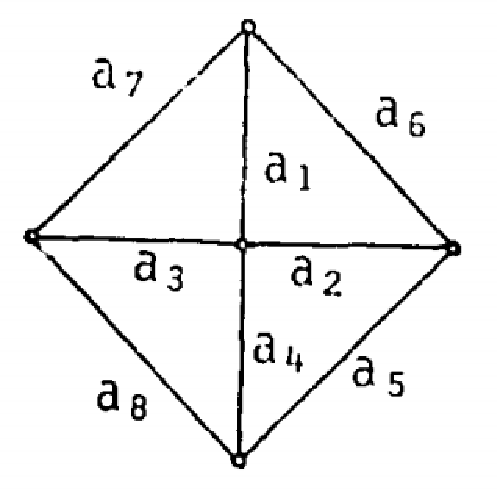
\includegraphics[width=\textwidth]{images/ceyhun-001-10-fig01}
    	\centering$Ç_2$ \\
    	\centering(a)
        \end{minipage}
        \begin{minipage}{0.32\textwidth}
	    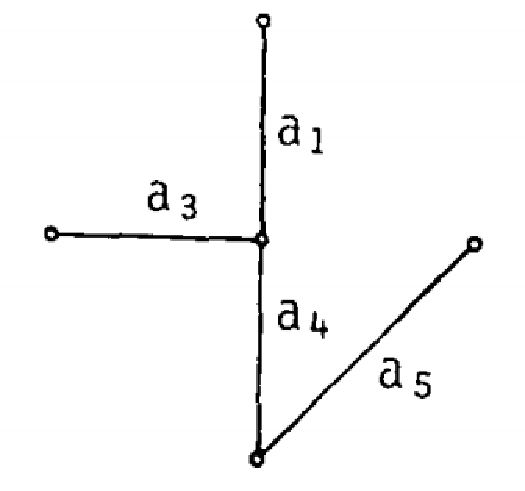
\includegraphics[width=\textwidth]{images/ceyhun-001-10-fig02}
	    \centering$Ç_1 \subset Ç_2$ \\
    	\centering(b)
        \end{minipage}
        \begin{minipage}{0.32\textwidth}
	    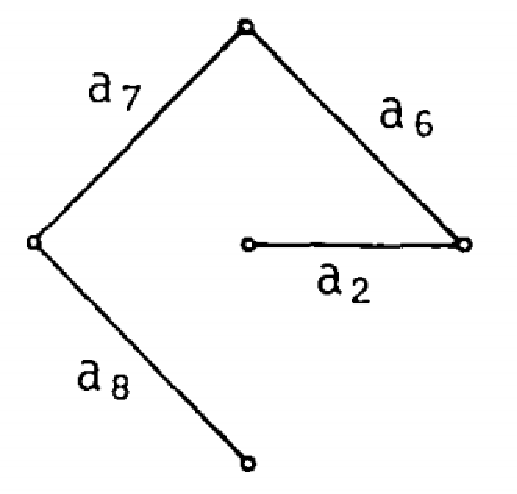
\includegraphics[width=\textwidth]{images/ceyhun-001-10-fig03}
	    \centering$Ç_1^T$ \\
    	\centering(c)
        \end{minipage}
	    \caption{Altçizge ve tümleraltçizge kavramlarının açıklanması.}
	    \label{fig:fig1}
\end{figure}
\end{document}